After initial testing, we recorded several detections. The results were not affected by the intensity of light in the room, suggesting that the detector was successfully optically sealed.

The muon flux detected is around 2.5 hits/minute, lower than in theory. We believe that this is due to our conservative data filtering, and small field of view: we wanted to reduce the chances of introducing noise as much as possible. As such, the calibration of our detector is crucial to capture accurate trajectories.


%oscilloscope 1
\begin{figure} [h]
    \centering
    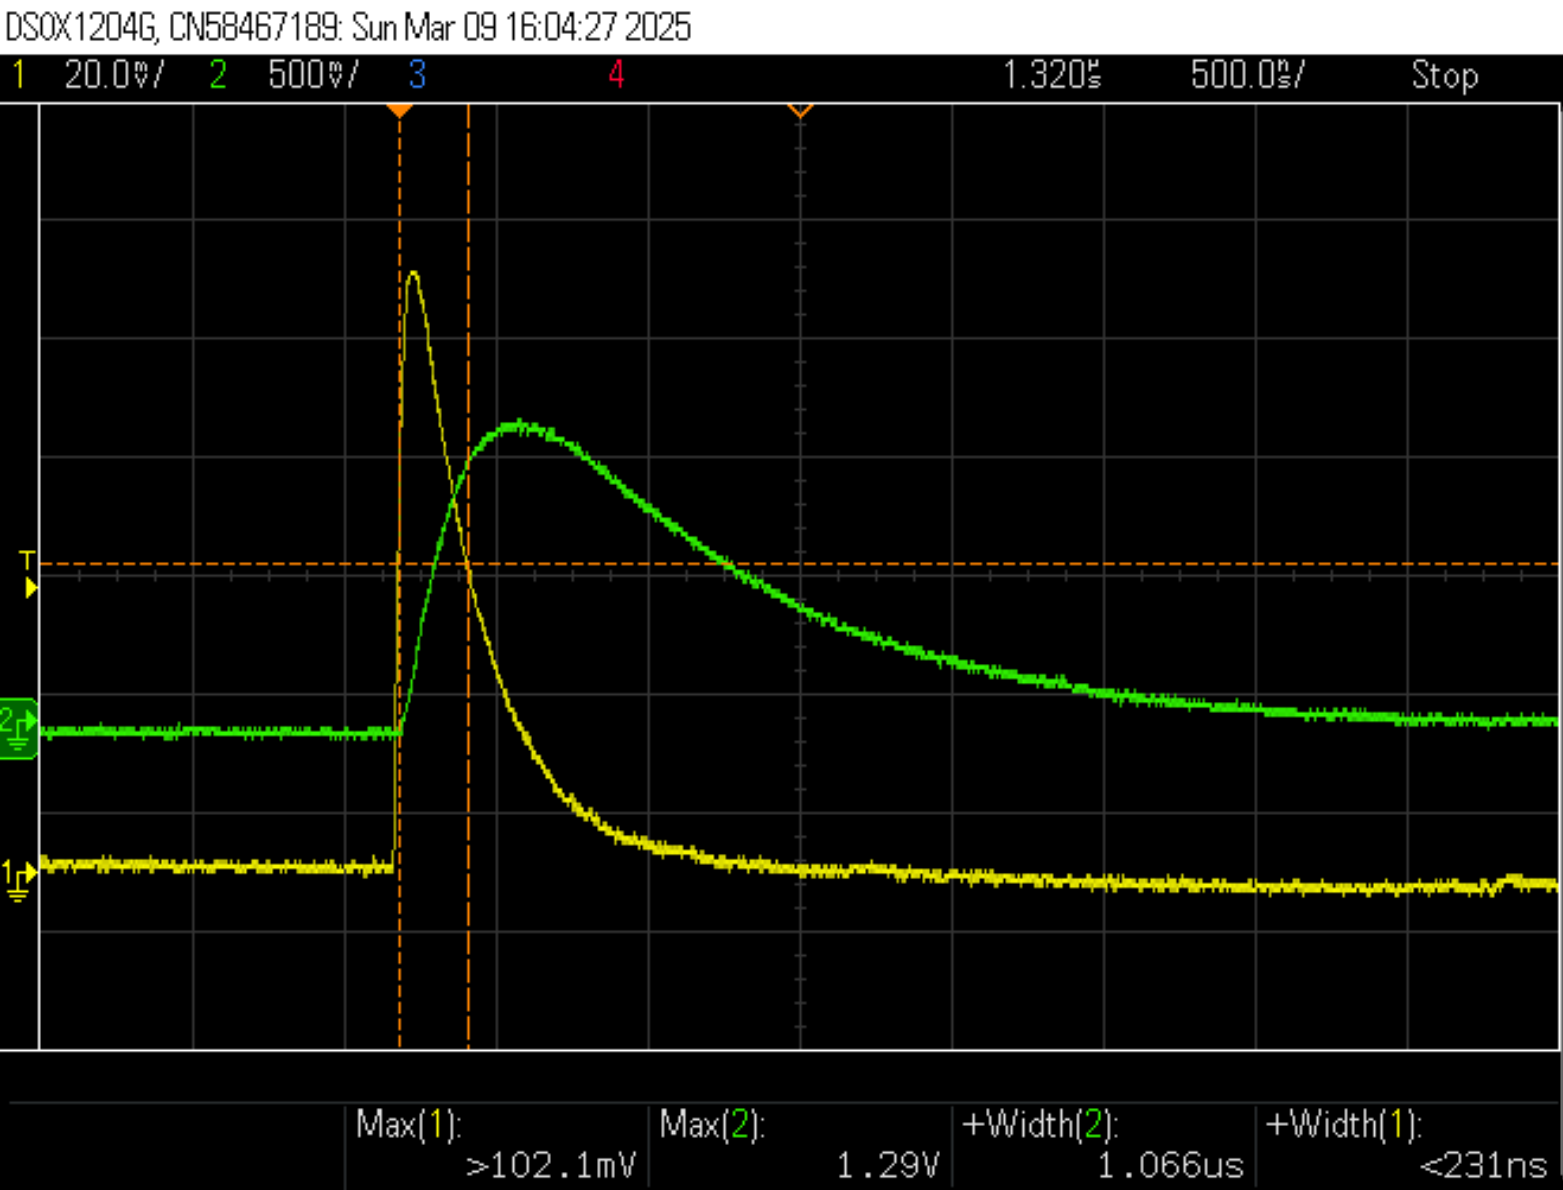
\includegraphics[width=0.58\linewidth]{figures/scope_yellow_green.png}
    \caption{Initial amplification testing with OnSemi C-Series SiPM (41\% photon detection efficiency (PDE), 420\,nm peak wavelength). \textbf{Yellow:} voltage across $49.9\,\Omega \pm 1\%$ shunt resistor on reverse-biased diode anode. \textbf{Green:} non-inverting op-amp configuration (LT1807) output. Light output measured from BC408 PVT scintillator.
}
    \label{fig3}
\end{figure}



%oscilloscope 2
\begin{figure} [h]
    \centering
    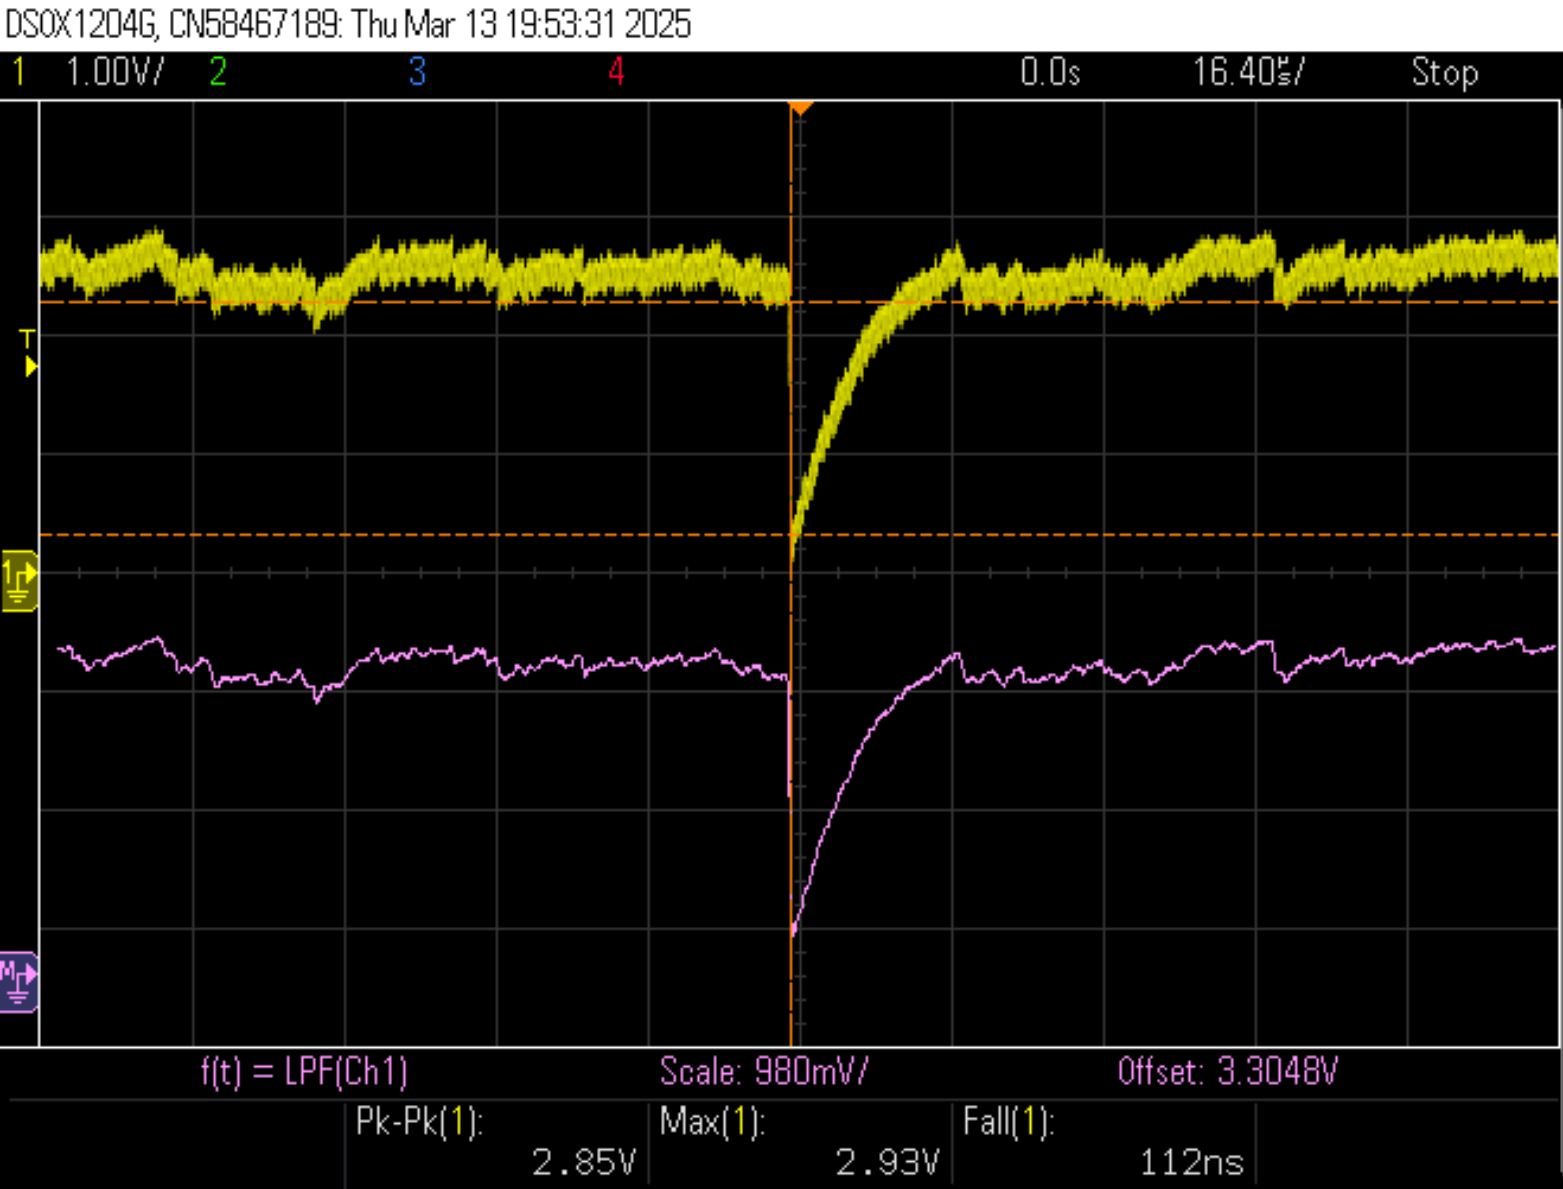
\includegraphics[width=0.58\linewidth]{figures/scope_yellow_purple.png}
    \caption{Initial transimpedance amplifier testing. Gain of $2.26 \times 10^5 \pm 1\%$. \textbf{Yellow:} inverting op-amp output. \textbf{Pink:} low-pass filter, 940\,kHz bandwidth.}
    \label{fig4}
\end{figure}

%Angle model
\begin{figure} [h]
    \centering
    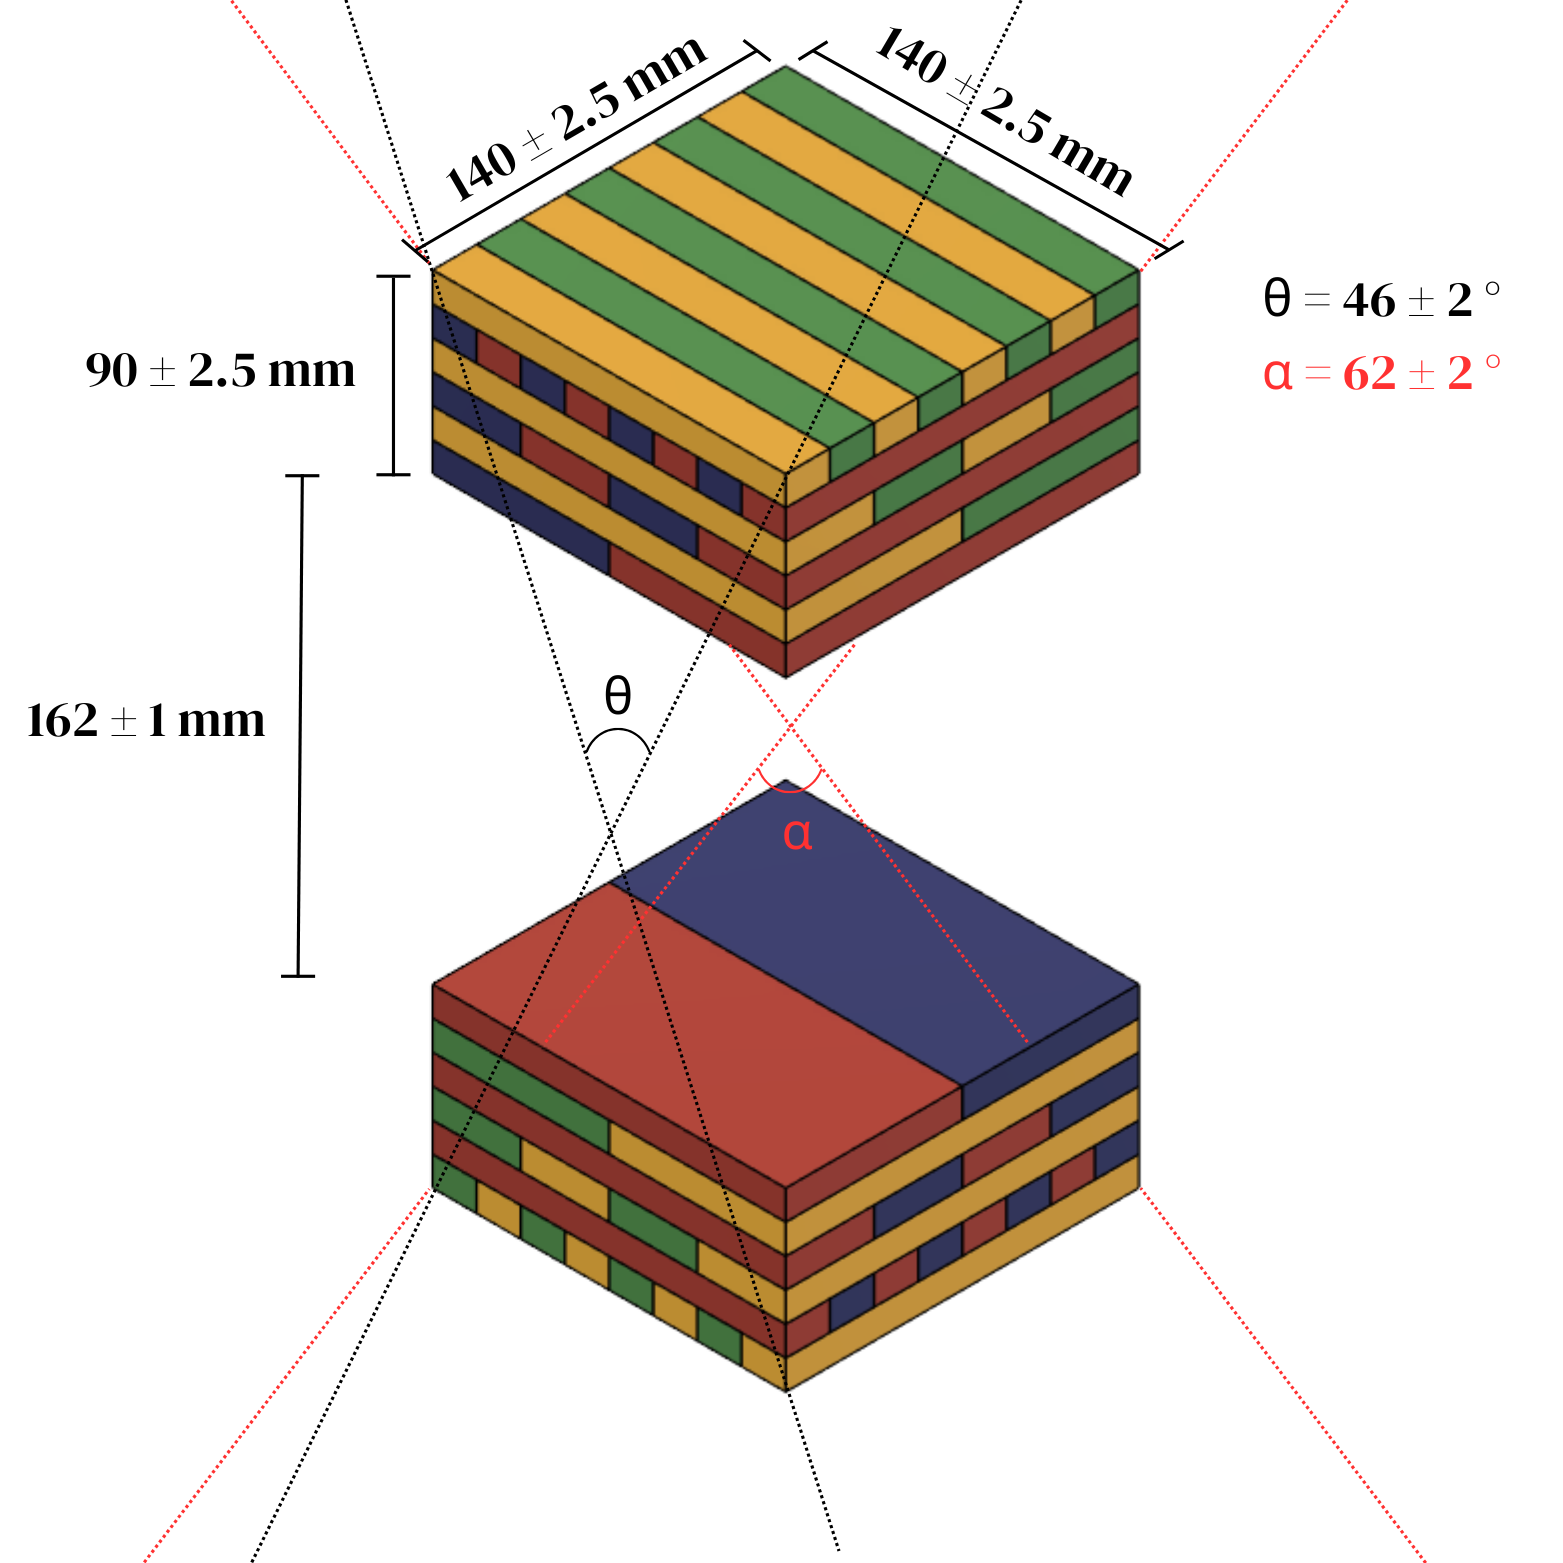
\includegraphics[scale=0.45]{figures/angle fig2.png}
    \caption{Cosmic ray capturing field of view: $46\pm2\degree$ minimum (on X and Y axes side projection), $62\pm2\degree$ maximum (on diagonal). Top and bottom scintillator stacks are $140\times140\times90 \pm2.5$ mm\textemdash separated by an air-gap of $162 \pm1$ mm. The minimum trajectory volume cross-section is $15\times15\text{ mm}: 225\text{ mm}^2$.}
    \label{angles}
\end{figure}

